\title{GraphQL in Cloud Computing}

\author{Averill Cate, Jr}
\affiliation{%
  \institution{The University of Indiana}
  \streetaddress{}
  \city{Bloomington} 
  \state{Indiana} 
  \postcode{47408}
}
\email{acate@iu.edu}

% The default list of authors is too long for headers}
\renewcommand{\shortauthors}{A. Cate, Jr}

\begin{abstract}
We are in the information age.  Possibly, the information overload age.
Data are the commodity of this technological era.  A significant number, if not
most of the world's industries are dependent on the internet and the exchange
of data.  It is reasonably safe to assume that how data are exchanged is
an important to understand.  Understanding data services have been changing
over time may be as vital as development of new tools and methods for data
exchange.  This paper will describe recent changes in tools and methods that
are used to facilitate the exchange of data in the information age.  This paper
will compare recent data service methods and briefly describe the costs and benefits
of each.
\end{abstract}

\keywords{hid505, GraphQL, Web Services, Cloud, Computing}

\maketitle

\section{Introduction}
Although data services and data exchange long pre-date the early 2000's.  The
volume of work that pre-dates 2000 would require volumes to adequately describe.
For clarity, this paper focuses on data services technologies that have emerged
since 2000 and the advent of Web 2.0 and in particular the data mining and
data sciences explosion that is taking place across the globe.

This paper will breifly describe two import exchange protocols, SOAP and REST.  
Next the paper will compare XML, a data format used in SOAP, with two data
formats used in REST, JSON, and GraphQL.  SOAP and REST are not the only
protocols that currently exist.  Nor are XML, JSON, and GraphQL the only data
formats that exist.  However, both protocols and all three formats are widely
used in academia and industry today and merit discussion.

\section{SOAP and XML}
SOAP is a XML-based data exchage protocol\cite{Quaine2007}.  SOAP stands for
``Simple Object Access Protocol``\cite{Microsoft2018}.  SOAP is a lightweight
protocol that, simply stated, is extensible and designed to facilitate the
exchange of structured data between disparate systems \cite{Microsoft2018}.
Etensible Markup Language (XML) is the structured data format that has been
used in conjuction with SOAP for data services \cite{Walsh1998}.  SOAP and XML
are still widely used today.  In some cases, due to legacy systems and security
concerns SOAP and XML are required for the use and development of data services.
An example of XML is shown in Figure~\ref{f:xml-example}
\cite{WikipidiaXML1028}.  An important point to note is, XML is a markup
language, which can be interpretted as a meta-language.  XML serves to not only
contain the data it delivered, but it also describes the data \cite{Aihkisalo2012}.

\section{REST and JSON}
Pautasso et. al. \cite{Pautasso2008} define REST as
Representational State Transfer.  REST was designed by Roy Fielding as part of his
doctoral dissertation while attending the University of California, Irvine
\cite{Fielding2000}.  Fielding developed REST in order to propose a framework
for and architecture that can be used in ``network-based application software``
\cite{Fielding2000}.  Fieldings work on REST occurred around 2000, but it has
only been in the last few years that we have seen the widespread implementation
of REST.  Figure~\ref{f:rest-example} we show an example of a REST/JSON data
packet.  The example could be the output from a query to a RESTful web service
or the input to be delivered to a RESTful web service that is meant to create
our update data.  JSON in comparison to XML is not a markup language.  In
comparison to XML, JSON is the data with some defining attributes, but it his
little, if any, meta-data that describe the data itself.  As an example, a JSON
data packet might have a list of users where each user object or item has a
first name attribute, last name attribute and an email address attribute with
values for each of those attributes, but the data packet itself, does not
describe the data format.  REST and JSON have also leant themselves towards the 
development of web-based Application Programming Interfaces (API).

\section{GraphQL}
SOAP and XML, REST and JSON have been part of the progression of the development
of web services and web APIs.  Some might say that the development of each
has revealed something new that has lead to the next technology
advancement in data services and data.  With the development of each technology
we also discover limitations of that new technology, which in-turn leads to the
next technological advancment.  For example, in industry, not long after SOAP
and XML became primary tools in web API development, some people began to
notice the difficulty in reading XML data in cases where developers need to
confirm data requests or data responses.  One might argue that using XML as the
data packet could have been an over extension of the use of XML in web
services.  In the mid to late 2000s REST and JSON based web services began to
take hold.  JSON may have been a better fit for web services and data mining
because formatting data to comply with a JSON data format focuses more on the
data itself than describing the data like XML does.  If true, and we conceed
that the format of JSON data rendered for situations where developers are trying
to test web services and the rendered data are easier to read then JSON may have
been the next logical step in the evolution of web services.  

Figure~\ref{f:wsdl-example} \cite{mycodde2016} is an example of the type of
interface developers and web service data consumers had to understand in order
to work effectively with SOAP/XML based web services.  Anyone trying to read
the WSDL document had to not only understand the nuances of things like XML,
namespacing, but also had to be able to understand how the web service's
operations were defined int the WSDL document.

Figure~\ref{f:swaggerui-example}\cite{swaggerio2018} is example of a REST/JSON web service
interface.  In comparison, it is easier to understand not only what proceedures
or methods the service provides, but as Figure~\ref{f:swaggerui-expansion}\cite{swaggerio2018}
demonstrates, it is easier to under stand the data types for the services input
parameters and resulting output data packets.  However, Figure~\ref{f:swagger-resp}\cite{swaggerresp2018}
provides an example of service  response from a REST/JSON based service and
although, visually, easier to understand compared XML.  It is challenging to
understand the relationships between the data set's components.  

\section{Figures}

In Figure~\ref{f:fly} we show a fly. Please note that because we use
just columwidth that the size of the figure will change to the
columnwidth of the paper once we change the layout to final. Changing
the layout to final should not be done by you. All figures will be
listed at the end.  Please do not use phrases such as \textit{shown in
  the figure below}. Instead use such as shown in Figure~\ref{f:fly}.

\begin{figure}[!ht]
  \centering\includegraphics[width=\columnwidth]{../../hid-sample/tex/images/fly.pdf}
  \caption{Example caption}\label{f:fly}
\end{figure}

To avoid copying the example figure in each hid directory, we actually
import it from the hid-sample directory. Lets assume you have a figure
in the image directory called myfigure.pdf. You can than replace the
line in the example with

\begin{verbatim}
\centering\includegraphics[width=\columnwidth]{images/myfigure.pdf}
\end{verbatim}

In case you use png than you must have a png that is at least 300dpi
(find out what that means and how to do that) and use 

\begin{verbatim}
\centering\includegraphics[width=\columnwidth]{images/myotehrfigure.png}
\end{verbatim}

When modifying the example, please do not check in the images from the
examples into your images directory as you will not need them for your
paper. Instead use images that you like to include. If you do not have
any images, do not palce anything in the images folder. However most
technologies could benefit for one image. Make sure you do not
plagiarize the image. Find out from the hand book how to do that. Any
plagiarism of images will result that we return the paper without
review as you have not understood how plagiarism works.

\section{Tables}

In case you need to create tables, you can do this with online tools
(if you do not mind sharing your data) such as
\url{https://www.tablesgenerator.com/} or other such tools (please
google for them). They even allow you to manage tables as CSV.

or generate them by hand while using the provided template in Table
\ref{t:mytable}. Note that
the caption is before the tabular environment.

\begin{table}[htb]
\centering
\caption{My caption}
\label{t:mytabble}
\begin{tabular}{lll}
1 & 2 & 3 \\
\toprule
4 & 5 & 6 \\
7 & 8 & 9
\end{tabular}
\end{table}

\section{Quotes}

Do not use double quotes \verb|"| but use \LaTeX\ ``quotes''. Quotes
{\bf MUST} not be used to highlight works. Quotes are {\bf STRICTLY}
used for quoting text from sources with citation following. If we find
a quote that is not followed by a citation we will return the paper
without review.

\section{Labels}

Do not use actual numbers in the taxt after you write for example
Figure 1 use the ref for the figure while using its label. In our
example it is Figure~\ref{f:fly} and Table Figure~\ref{t:mytabble}.
See the source for the example.

\section{Footnotes}

Footnotes must be avoided in papers. All URLs must be included as full
references and citations and used with the \verb|\cite| command
\footnote{do not use footnotes}. You {\bf must} not use urls in the
text or paper.

\section{Plagiarism}

The class includes a section about plagiarism which you must adhere
to. Copying text without proper citation is considered cheating and we
will assign the grade ``F'' for the paper if we find you do it. It is
in your responsibility to make sure plagiarism does not occur. Please
be aware that our checks are better than the once provided by turnitin
or other online checkers. Excuses such as ``I did not have time'' or
``I forgot'' can not apply as you have enough time to prepare the
paper and must not forget. 

\section{Check}

make sure just as in previous assignments that you check your paper
with chktex and lacheck. Fix the errors that you see. Some of the
errors may be ok, but in general make sure you address all of them. If
in doubt work with the TA. Simply use

\begin{verbatim}
make check
\end{verbatim}

We include in the handbook a list with common issues that we see when
students submit papers. One particular important issue is not to use
the underscore in bibtex labels. It is your responsibility to check
the paper for the issues indicated.

To check bibliographies simply use

\begin{verbatim}
pdflatex report
bibtex report
\end{verbatim}

You will see the errors and warning son the screen address them

TA's will in addition use a special test checking for additional
format issues such as detecting if you used labels and refs for
floats. You are welcome to also try this test, but we provide it
without explanation as no explanation is needed since if you followed
the instructions on floats there should be no issues. If you like to
do that test, you can use  

\begin{verbatim}
make check-ta
\end{verbatim}

\section{Convenient Setup}

If you do not have already a paper dir in your repository, here is a
way to create one. Replace the hid-sp18-000 with your hid.

\begin{verbatim}
export HID=hid-sp18-000
mkdir -p ~/github/cloudmesh-community
cd ~/github/cloudmesh-community
git clone https://github.com/cloudmesh-community/hid-sample.git
git clone https://github.com/cloudmesh-community/$HID.git
\end{verbatim}

Next copy the paper example

\begin{verbatim}
cp -r hid-sample/paper $HID
cd $HID
git add paper
git commit -m "add the paper directory" paper
git push
\end{verbatim}

Make sure there is no \verb|/| behind the paper in the cp command or you mess up the
copy process.


\section{Creating the PDF}

The PDF\ can be created simply with 

\begin{verbatim}
make clean
\end{verbatim}



{\bf UNDER NO CIRCUMSTANCES ARE YOU ALLOWED TO CHECK IN YOUR PDF OR
  TEMPORARY LATEX FILES INTO GITHUB. GIT NEEDS TO STAY CLEAN AND ONLY
  CONTAIN THE SOURCES.}

We will deduct points if you do violate this.

\section{Conclusion}

Put here an conclusion. Conclusion and abstracts must not have any
citations in the section.


\begin{acks}

  The authors would like to thank Dr.~Gregor~von~Laszewski for his
  support and suggestions to write this paper.

\end{acks}

\bibliographystyle{ACM-Reference-Format}
\bibliography{report} 

\begin{figure}[!ht]
  \centering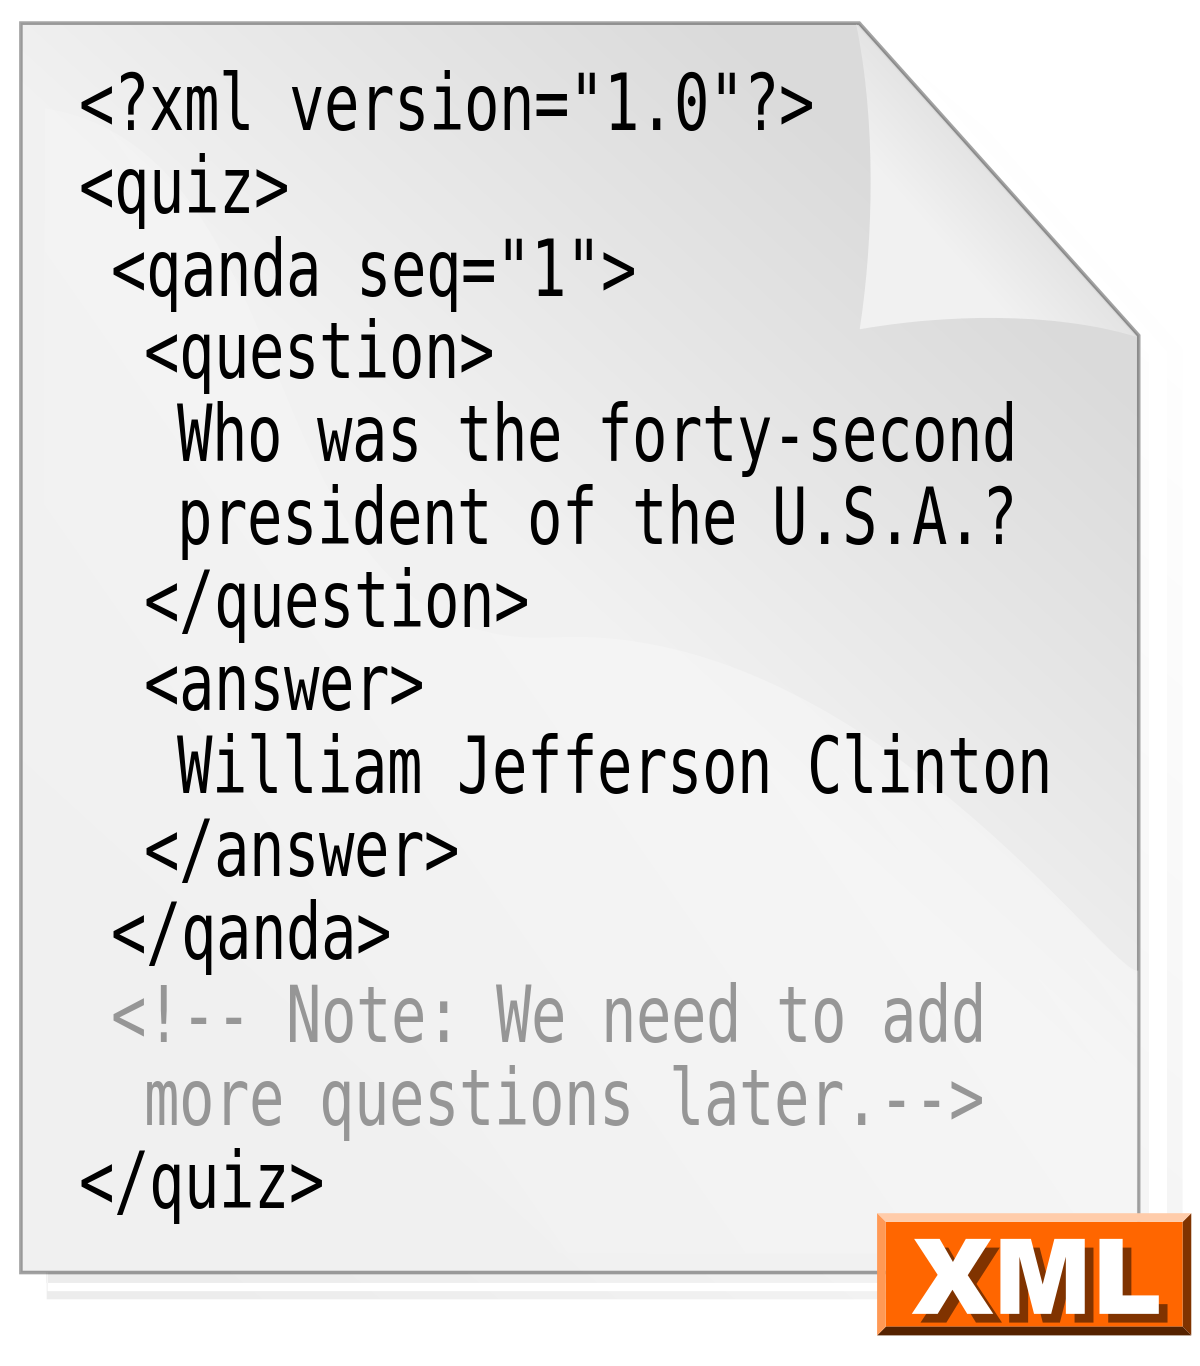
\includegraphics[width=\columnwidth]{images/xml-example.png}
  \caption{SOAP/XML Example}\label{f:xml-example}
\end{figure}

\begin{figure}[!ht]
  \centering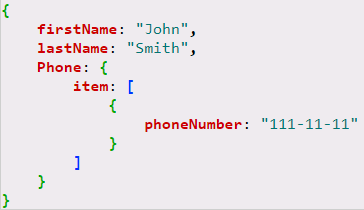
\includegraphics[width=\columnwidth]{images/json-rest-example.png}
  \caption{REST/JSON Example}\label{f:rest-example}
\end{figure}

\begin{figure}[!ht]
  \centering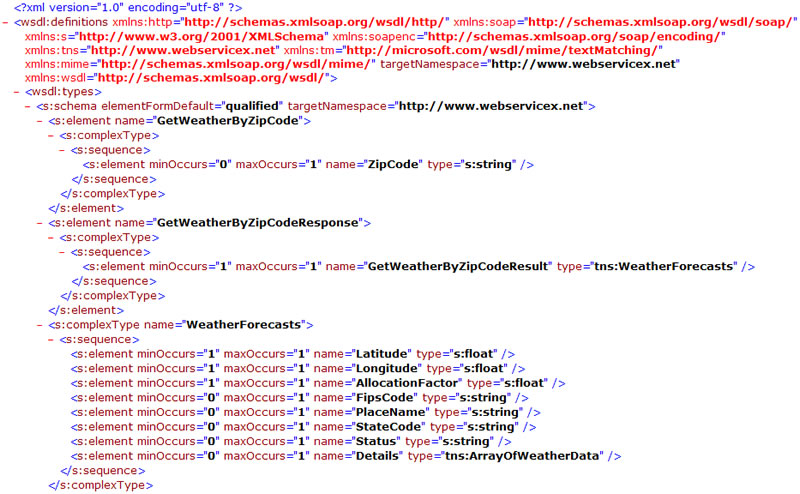
\includegraphics[width=\columnwidth]{images/wsdl-example.jpg}
  \caption{WSDL Example}\label{f:wsdl-example}
\end{figure}

\begin{figure}[!ht]
  \centering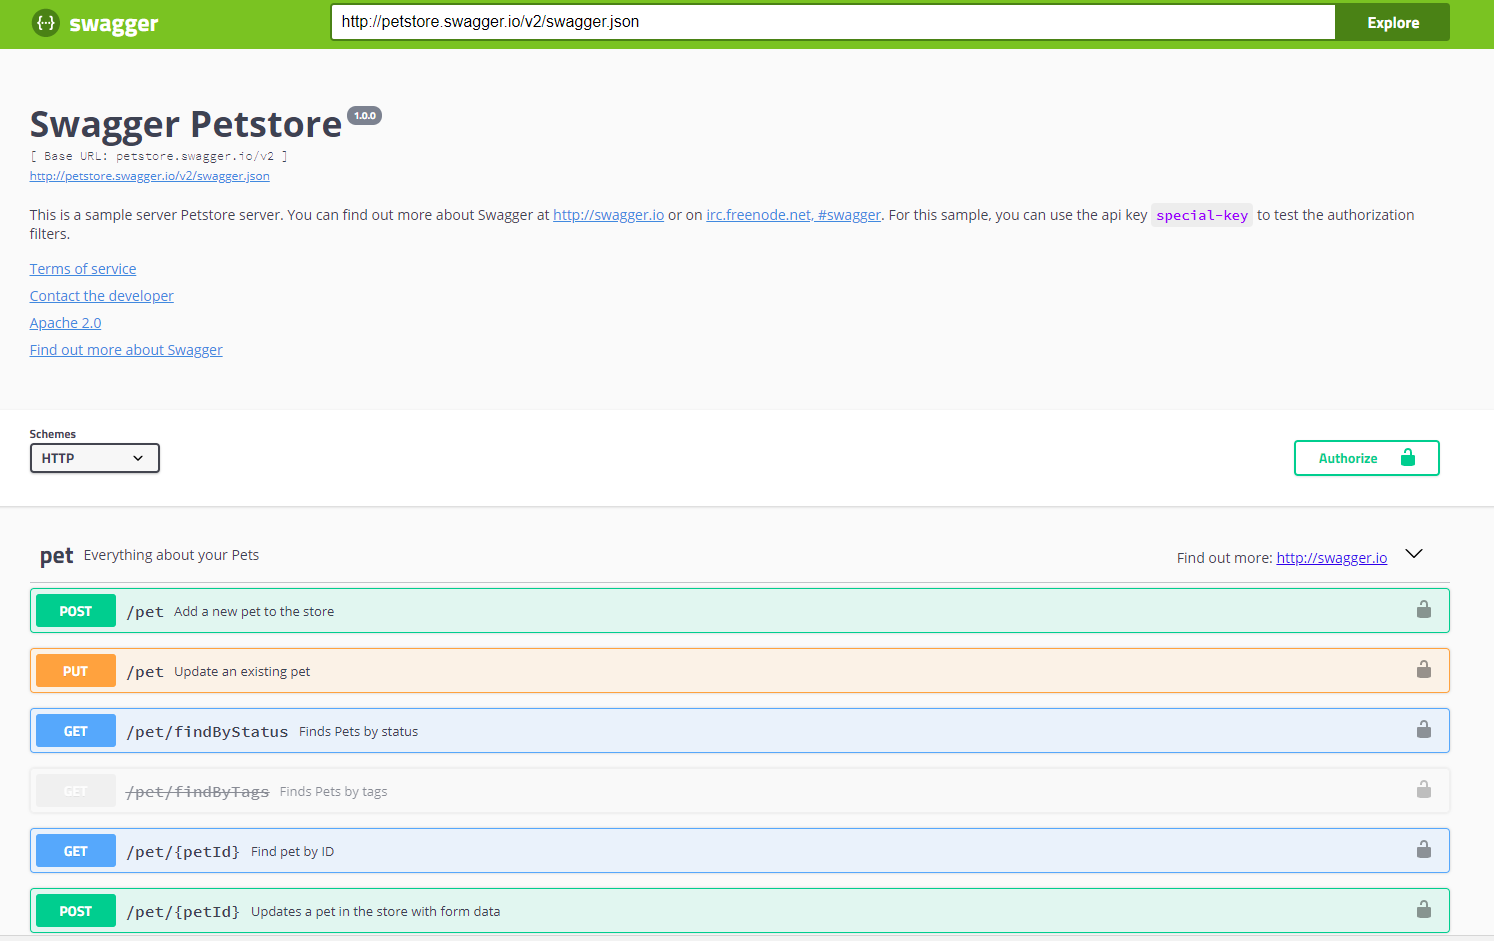
\includegraphics[width=\columnwidth]{images/swaggerui.png}
  \caption{Swagger UI Example}\label{f:swaggerui-example}
\end{figure}

\begin{figure}[!ht]
  \centering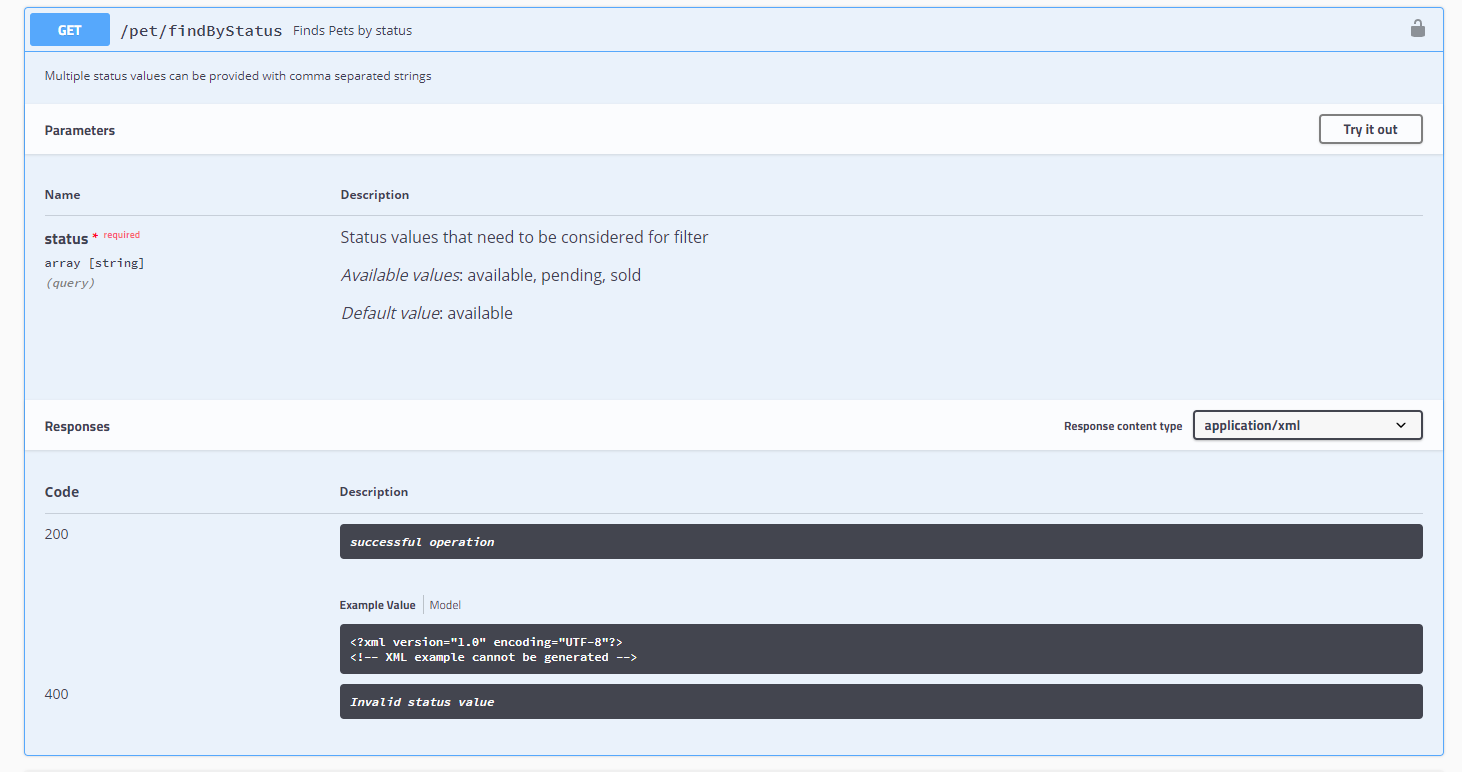
\includegraphics[width=\columnwidth]{images/swaggerui-expansion.png}
  \caption{Swagger UI Expanded}\label{f:swaggerui-expansion}
\end{figure}

\begin{figure}[!ht]
  \centering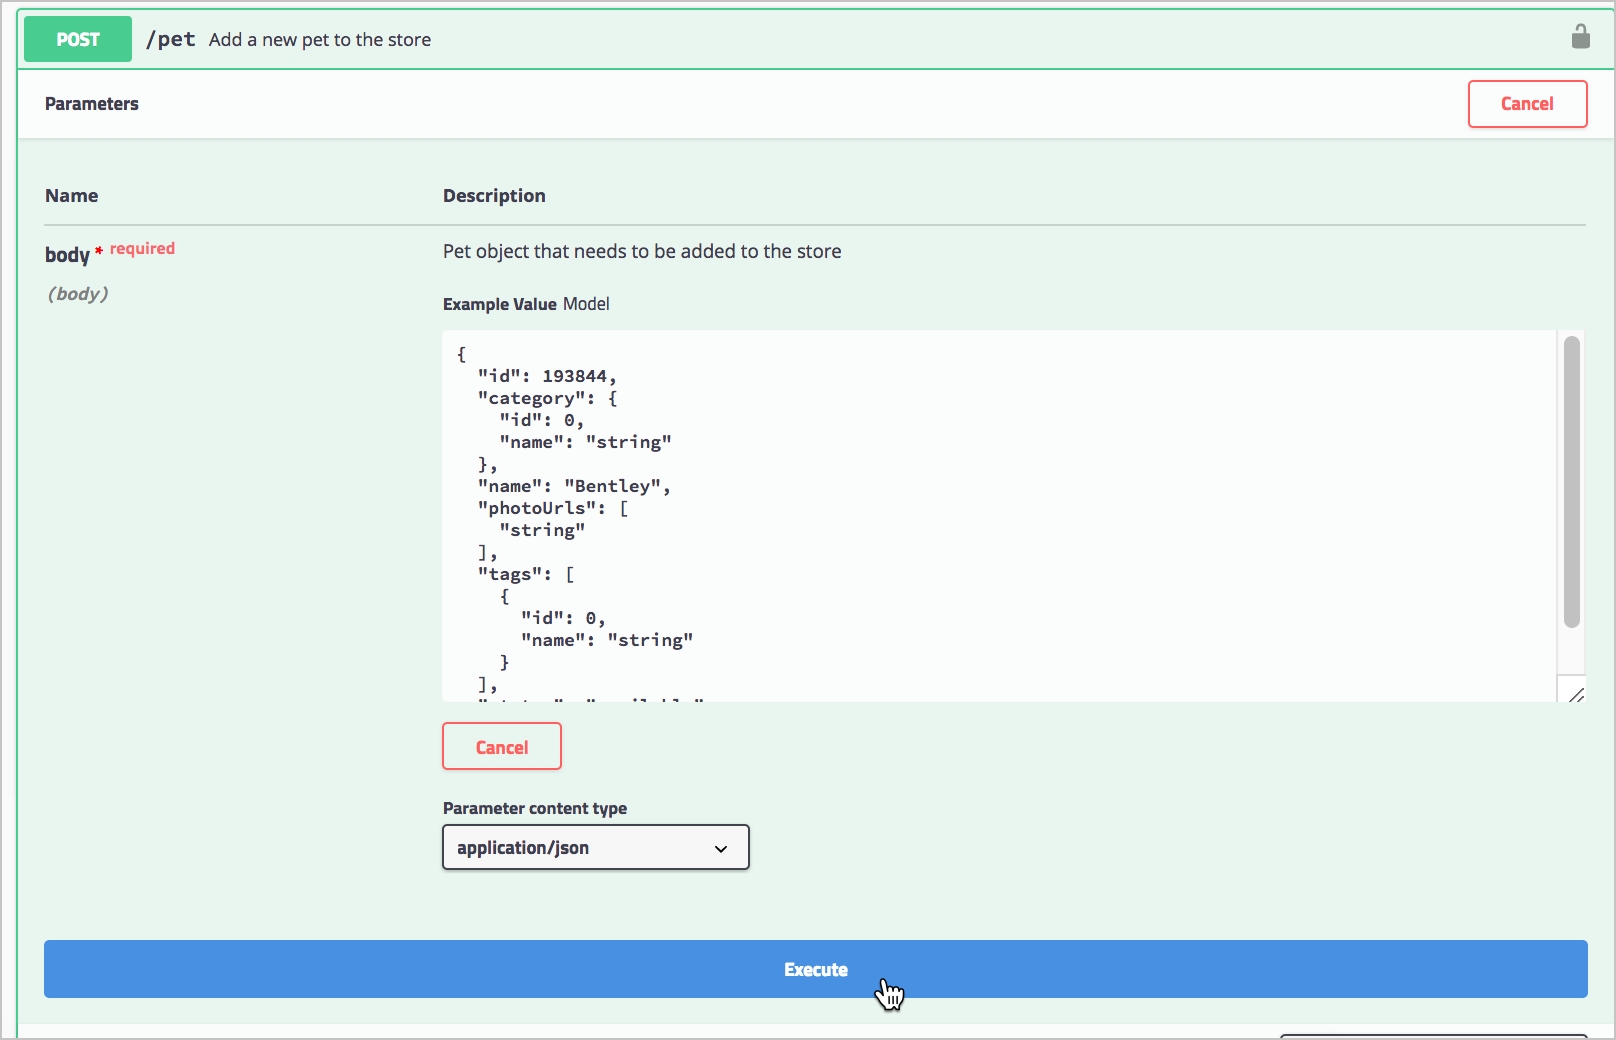
\includegraphics[width=\columnwidth]{images/swaggerui_execute.png}
  \caption{Swagger UI Response}\label{f:swagger-resp}
\end{figure}
